% DO NOT COMPILE THIS FILE DIRECTLY!
% This is included by the other .tex files.

\begin{frame}[t,plain]
\titlepage
\end{frame}

\begin{frame}
    \frametitle{Bringing workflows into threat intelligence platform}
    After multiple years, MISP users have reach a significant maturity level:
    \begin{itemize}
        \item Events with {\bf complex TTPs, objects and attributes};
        \item Exhaustive context such as {\bf MITRE ATT\&CK}, tags and relationships;
        \item Availability of {\bf external modules and services} (e.g. from expansion services to third-party CTI);
        \item Comprehensive {\bf processing pipelines} for threat intelligence are available;
    \end{itemize}
\end{frame}

\begin{frame}
    \frametitle{Where is the glue?}
    \begin{itemize}
        \item Initial idea came from GeekWeek7.5
        \begin{center}
            
\includegraphics[width=0.5\linewidth]{pictures/geekweek75.jpg}
        \end{center}
    \item Experienced users wanted to have a way to {\bf trigger actions and to modify to behavior of MISP} and especially leveraging what they have in their MISP platform.
    \item {\bf Creating workflows for any of the steps} in MISP (creating attributes/objects, publishing and sharing information, ...). 
    \end{itemize}
\end{frame}

\begin{frame}
    \frametitle{Simplistic overview}
    \begin{enumerate}
        \item \textbf{User Interacts} with MISP using the UI or API
        \item MISP handles the request, starts \textbf{preparing data} to perform the operation
        \item MISP checks if there are workflows \textbf{listening to the trigger}
        \item MISP fetches enabled workflows and \textbf{executes} them
        \item If all went fine, MISP \textbf{continue} to perform the operation
    \end{enumerate}
\end{frame}


\begin{frame}
    \frametitle{Terminology}
    \begin{enumerate}
        \item \textbf{workflow}: Sequence of actions to be executed
        \item \textbf{execution path}: A path composed of actions to be executed sequentially
        \begin{itemize}
            \item A workflow can contain more than one execution path
        \end{itemize}
        \item \textbf{trigger}: Starting point of an \texttt{execution path}. Triggers are called when specific action are done by MISP
        \begin{itemize}
            \item A workflow can contain more than one trigger, but only one per type
        \end{itemize}
    \end{enumerate}
    \begin{center}
        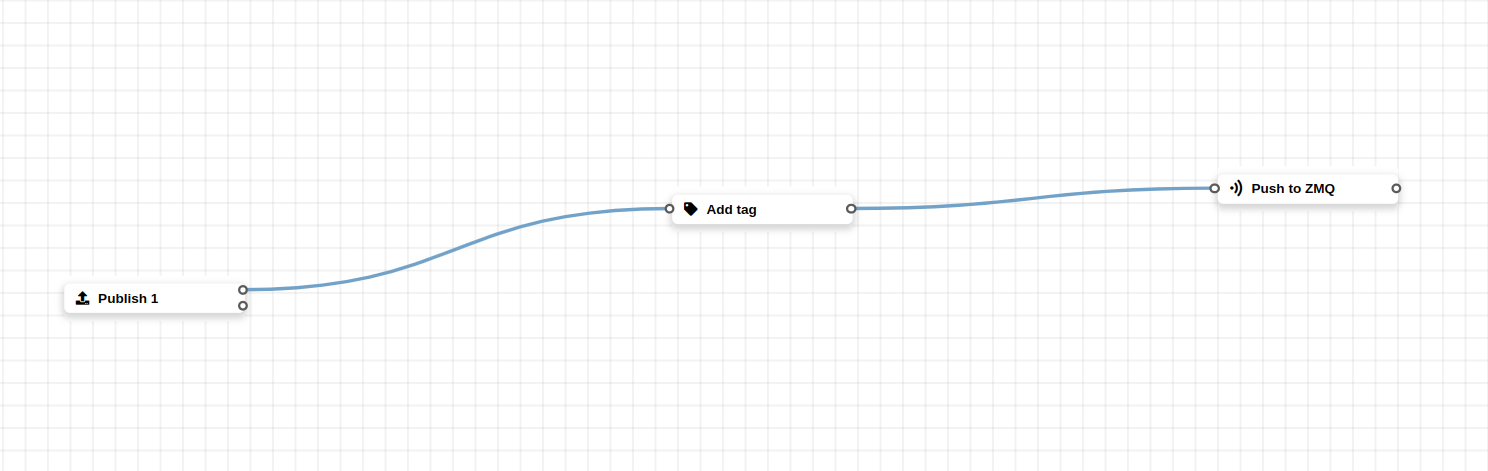
\includegraphics[width=1.0\linewidth]{pictures/workflow-view.png}
    \end{center}
\end{frame}


\begin{frame}
    \frametitle{Workflow execution in MISP}
    \begin{enumerate}
        \item A trigger is called;
        \item Collect workflows listening to called trigger;
        \item Execute workflows in the saved order;
    \end{enumerate}
    \begin{center}
        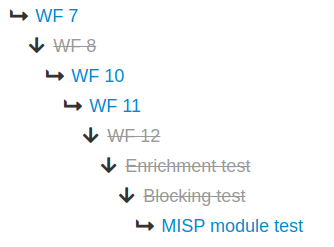
\includegraphics[width=0.5\linewidth]{pictures/execution-order-1.png}
    \end{center}
\end{frame}

\begin{frame}
    \frametitle{Execution Paths}
    Currently 2 types of execution path:
    \vspace{0.5em}
    \begin{itemize}
        \item {\bf Blocking}: Execution is stoped in case of error
        \begin{itemize}
            \item Current workflow's blocking execution path is {\bf stopped}
            \item Any other blocking path of next workflows {\bf will not be executed}
        \end{itemize}
        \vspace{0.5em}
        \item {\bf Non-blocking}/Deferred: Stop execution for current path only
        \begin{itemize}
            \item Current execution path is {\bf stopped}
            \item {\bf Resume} execution of remaining paths
            \item Paths from other workflow will be {\bf executed}
        \end{itemize}
    \end{itemize}
\end{frame}

\begin{frame}
    \frametitle{Execution Order and Execution Types}
    \begin{itemize}
        \item \textbf{Blocking} paths from all workflows are executed first in the saved order
        \item If any blocking executions failed, the action that called the trigger will \textbf{be stopped}
        \item \textbf{Parallel/Deferred} paths from all workflows are executed. The order is irrelevant
    \end{itemize}

    \begin{center}
        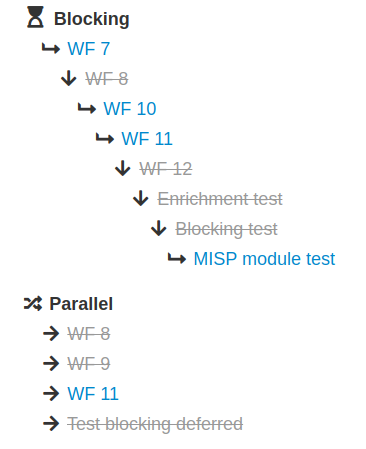
\includegraphics[width=0.35\linewidth]{pictures/execution-order-2.png}
        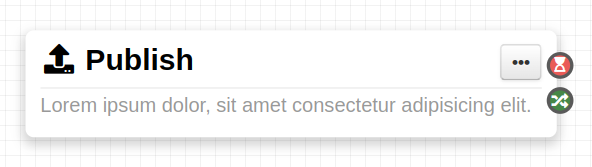
\includegraphics[width=0.40\linewidth]{pictures/trigger-outputs.png}
    \end{center}
\end{frame}

\begin{frame}
    \frametitle{Publishing example}
    Example:
    \begin{enumerate}
        \item An Event is published
        \item MISP starts the publishing process
        \item MISP executes a workflow listening to the trigger
        \begin{itemize}
            \item {\bf execution success}: Proceed publishing
            \item {\bf execution failure}: Stop publishing, log the reason and report the failure to the user
        \end{itemize}
    \end{enumerate}
\end{frame}

\begin{frame}
    \frametitle{Execution context}
    \begin{itemize}
        \item Workflow can be triggered by any users
        \item However, the user for which the workflow executes is the workflow creator
        \item This is to make sure users with a higher privilege will have their workflow correctly executed
    \end{itemize}
\end{frame}

\begin{frame}
    \frametitle{Workflow modules}
    \begin{center}
        
\includegraphics[width=0.5\linewidth]{pictures/module-type.png}
    \end{center}
    \begin{itemize}
        \item 3 types of modules
        \begin{itemize}
            \item \texttt{trigger}: Entry point of the execution
            \begin{itemize}
                \item Event publish, email about to be sent, feed data about to be saved, ...
            \end{itemize}
            \item \texttt{logic}: Allow to redirect the execution flow.
            \begin{itemize}
                \item IF condition, fork the blocking execution into a non-blocking one, ...
            \end{itemize}
            \item \texttt{action}: Modules that can modify data, prevent execution or perform additional actions
            \begin{itemize}
                \item Publish to ZMQ, perform enrichments, block the execution, ...
            \end{itemize}
        \end{itemize}
    \end{itemize}
\end{frame}


\begin{frame}
    \frametitle{Creating a workflow with the editor}
    \begin{enumerate}
        \item Drag a \texttt{trigger} module from the side panel to the canvas
        \item Drag an \texttt{action} module from the side panel to the canvas
        \item From the \texttt{trigger} output, drag an arrow into the \texttt{action} input (left side)
        \begin{itemize}
            \item You can choose between a \texttt{blocking} and \texttt{non-blocking} execution path by using the associated trigger output
        \end{itemize}
    \end{enumerate}
    \begin{center}
        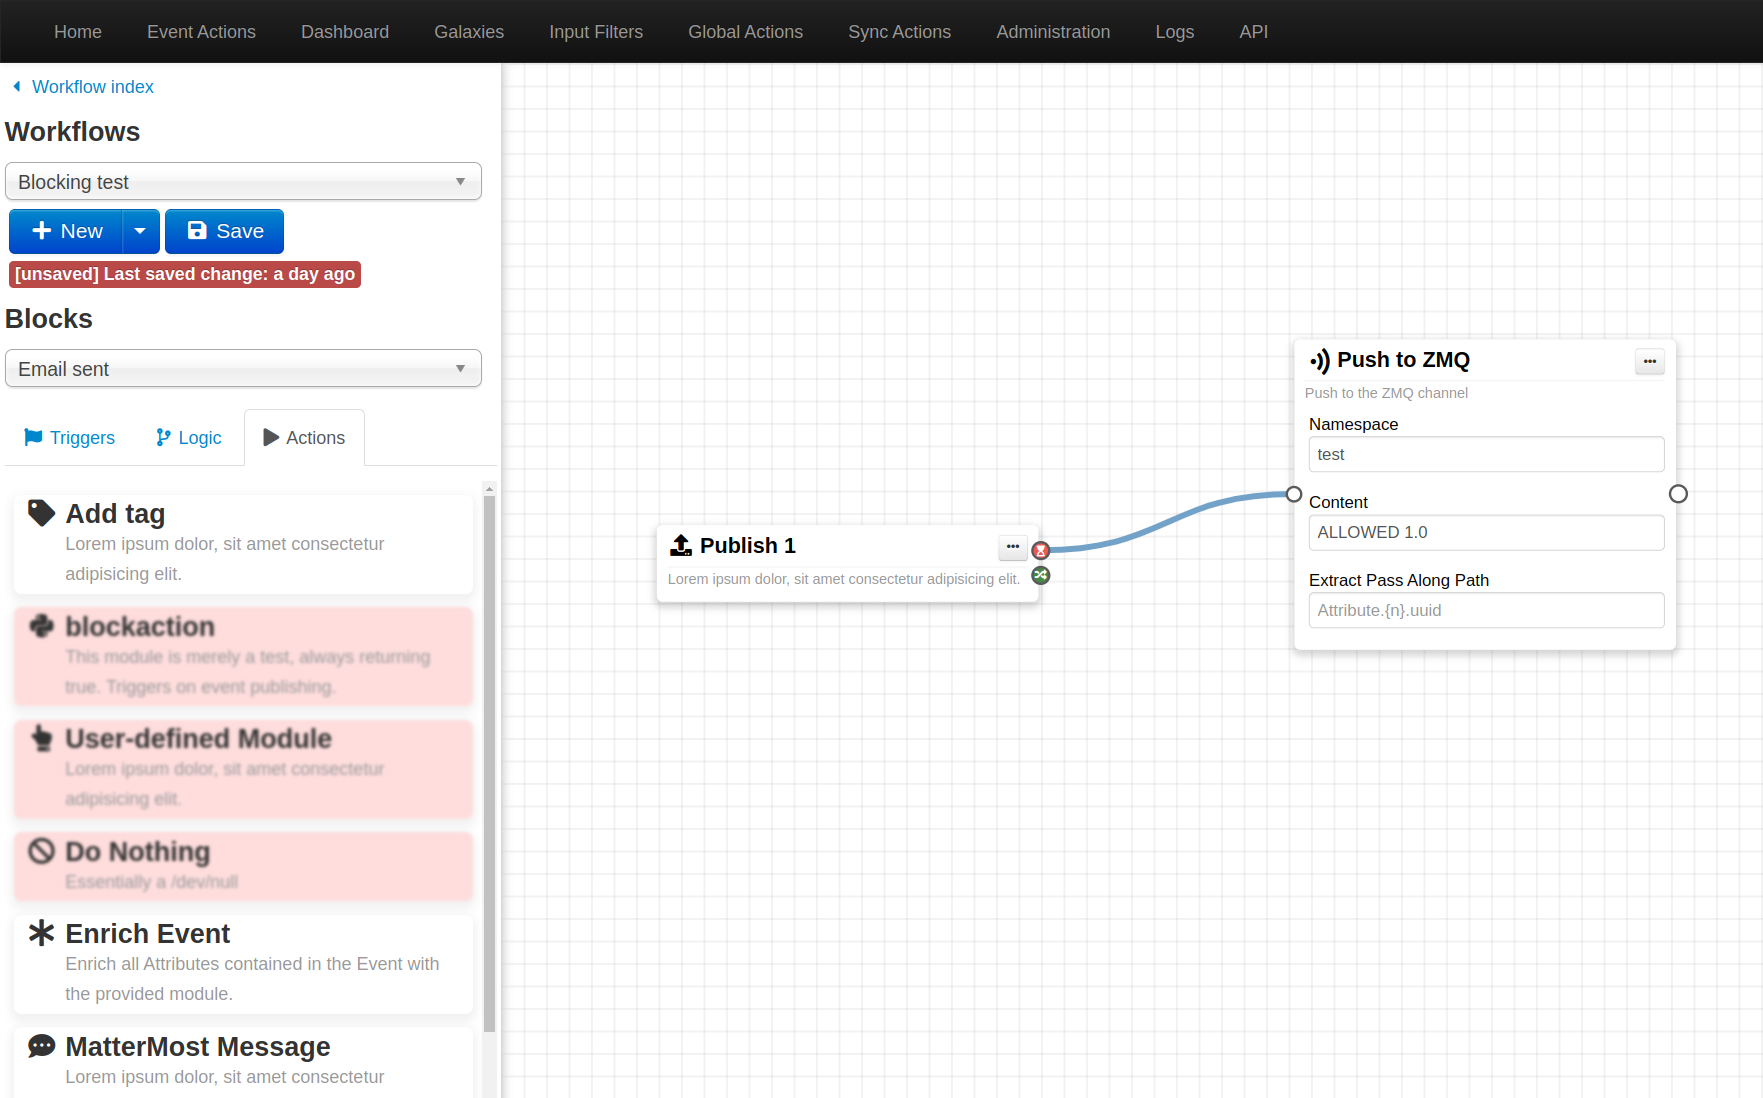
\includegraphics[width=1.0\linewidth]{pictures/editor-1.png}
    \end{center}
\end{frame}


\begin{frame}
    \frametitle{Workflow example with ATT\&CK}
    \begin{center}
        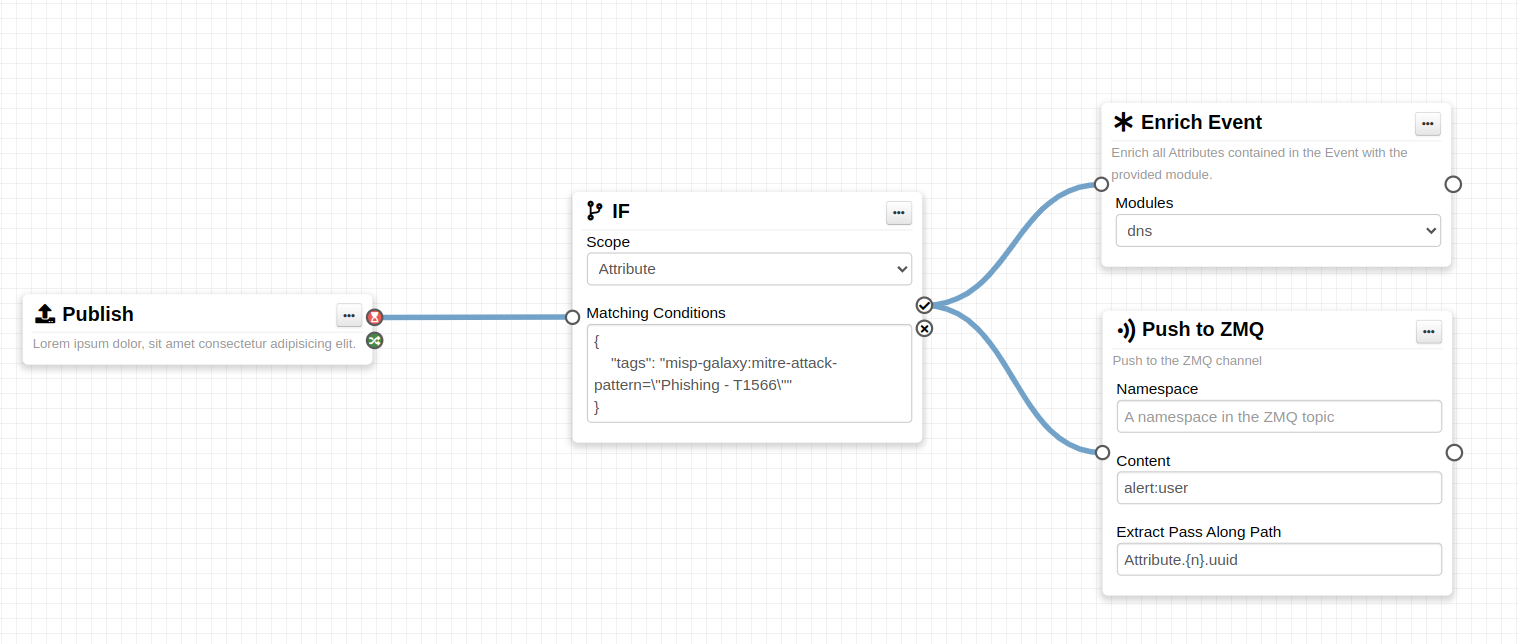
\includegraphics[width=0.9\linewidth]{pictures/ATT&CK-support.png}
    \end{center}

    \begin{enumerate}
        \item Automatically processing phishing cases from ATT\&CK context including enrichments and publishing pipelines. 
    \end{enumerate}
\end{frame}


\begin{frame}
    \frametitle{Workflow - advanced example}
    \vspace{-2em}
    \begin{center}
        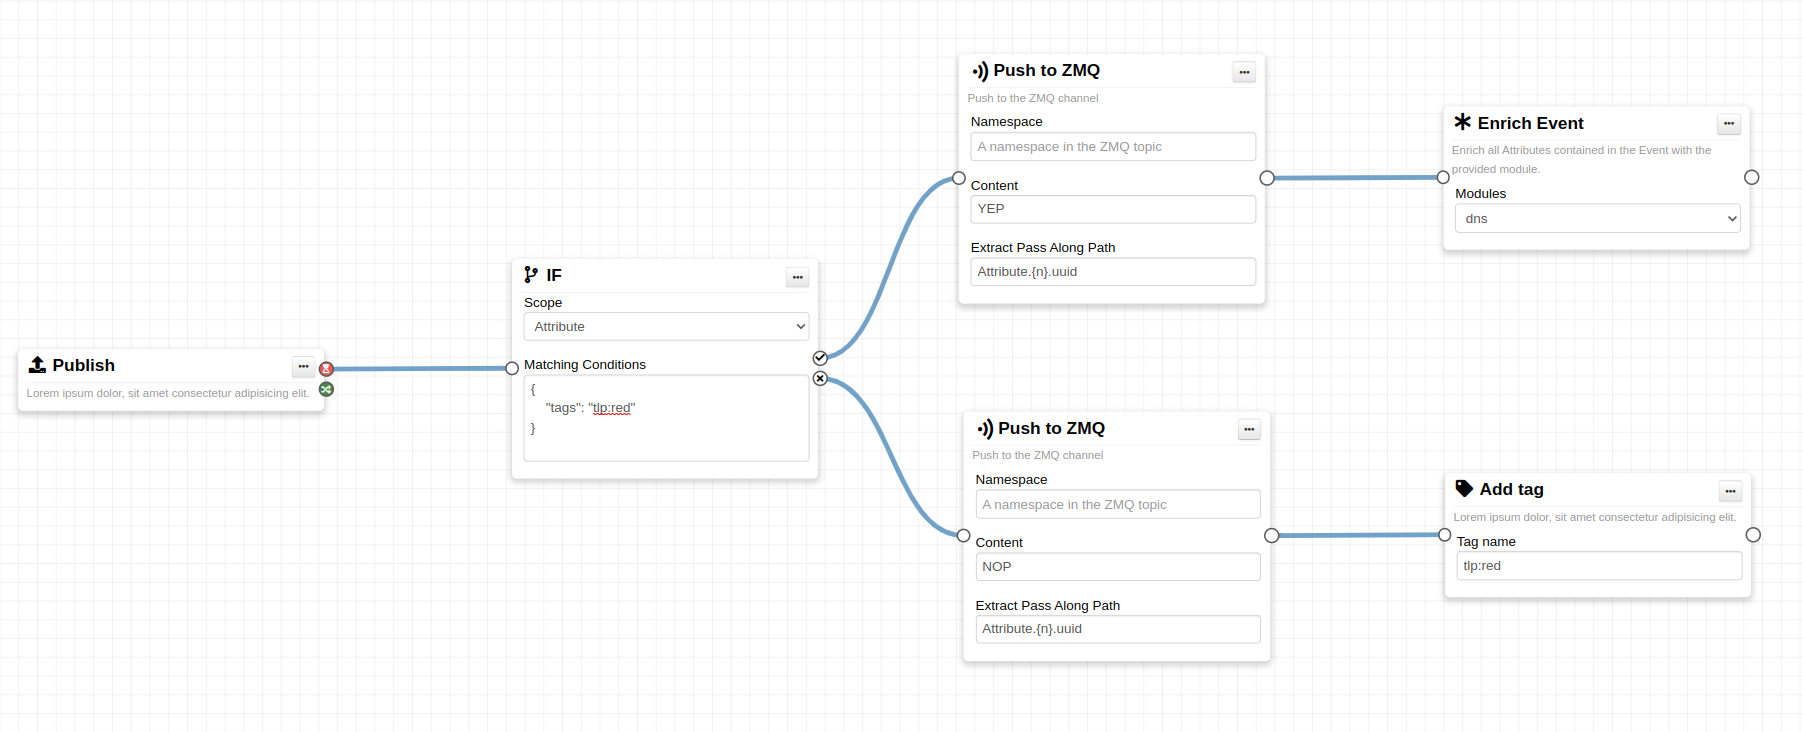
\includegraphics[width=1.05\linewidth]{pictures/example-7.png}
    \end{center}
    \begin{center}
        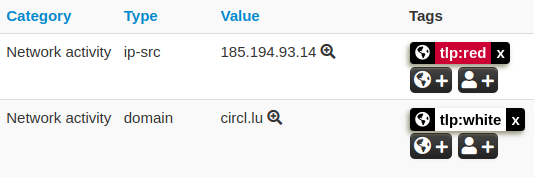
\includegraphics[width=0.45\linewidth]{pictures/event-1.png}
    \end{center}
\end{frame}

\begin{frame}
    \frametitle{Ongoing developments}
    \begin{itemize}
        \item First release of the workflow in MISP for the FIRST.org annual conference in Dublin (end of June).
        \item {\bf Workflows are shareable} and a library of workflows will be available.
        \item Gathering ideas and requirements for new workflows from the threat intelligence community.
        \item Reviewing ATT\&CK techniques to be mapped in the MISP workflows.
    \end{itemize}
\end{frame}

